\documentclass{beamer}
\usetheme{boxes}
\setbeamerfont{title}{family=\rm}
\usefonttheme{serif}
\usepackage{graphicx, float}
\usepackage{amsmath, amssymb}
\usepackage{listings}
\usepackage{pgfpages}
%\setbeameroption{show notes}
\setbeameroption{show notes on second screen=right}
\graphicspath{{Figures/}}

\title{Large-scale structure of complex networks (Part 2)}
\author{\small Snehal M. Shekatkar}
\institute{Centre for modeling and simulation,\\  S.P. Pune University, Pune}
\date{}

\begin{document}
%-------------------------
\begin{frame}
    \maketitle
    \note<1>{Hello}
\end{frame}
%-------------------------
%-------------------------
\begin{frame}
    \frametitle{Community structure in networks}
    \centering
    \note<1>{Network of coauthorships in a university department}
    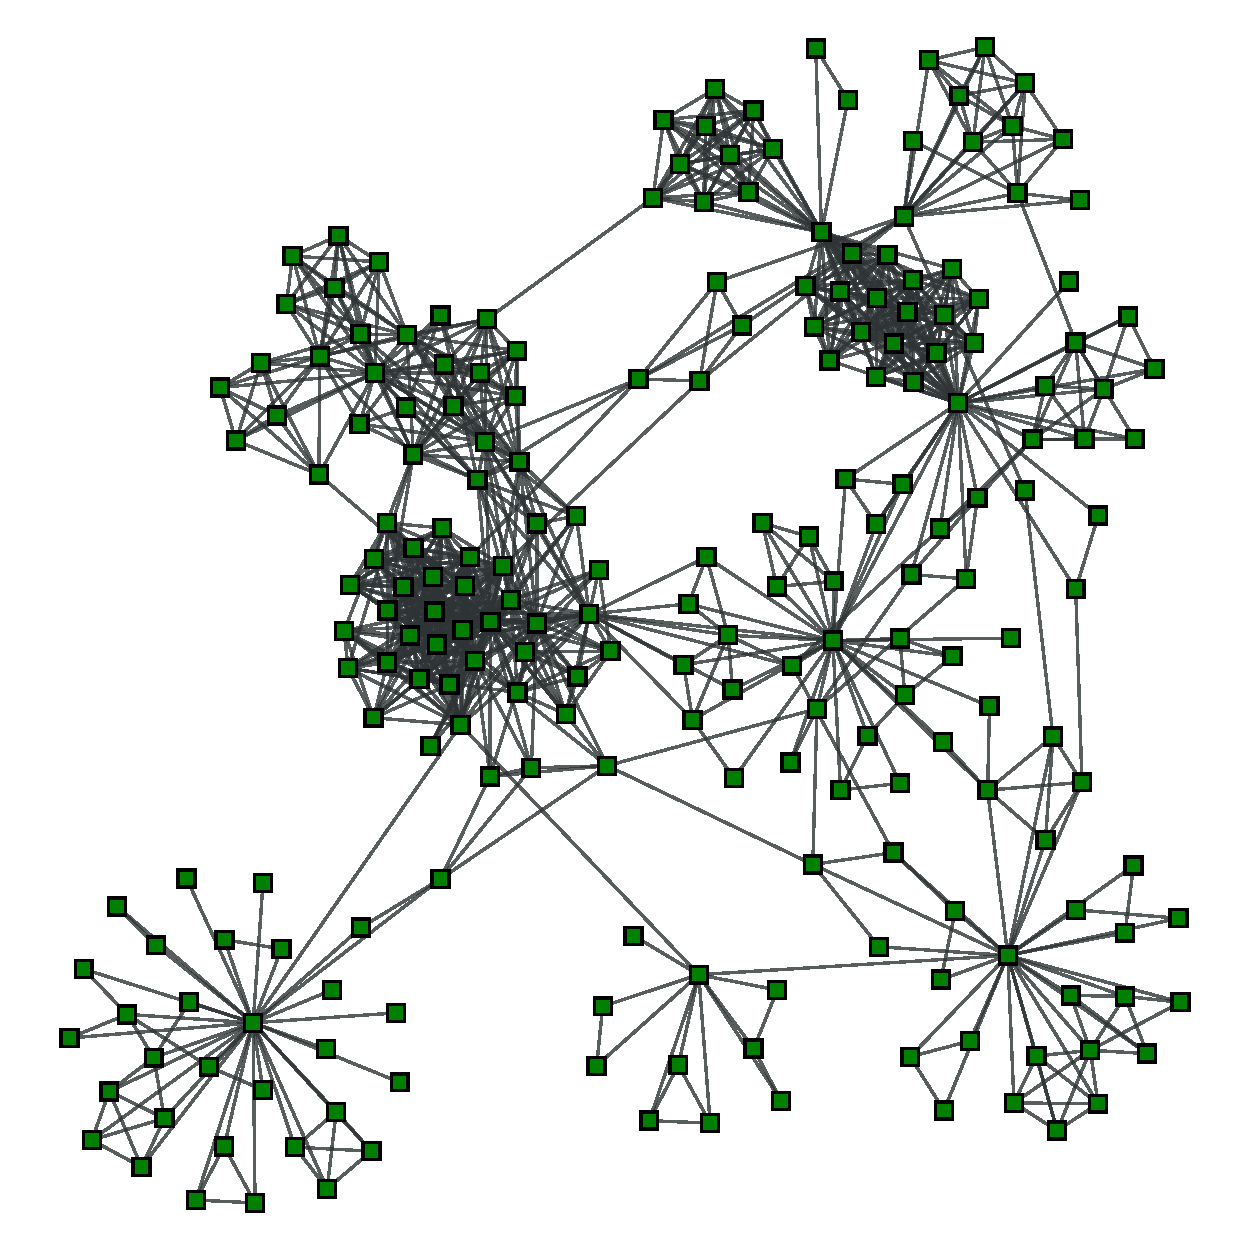
\includegraphics[width=0.8\columnwidth]{coauthors.pdf}
\end{frame}
%-------------------------
%-------------------------
\begin{frame}
    \frametitle{Community structure in networks}
    \centering
    {\bf What are communities?}
    \vspace{2em}
    \begin{itemize}
    \setlength\itemsep{1em}
        \item{{\bf Traditional definition}: Groups of nodes with a high internal link density}
        \item{{\bf Modern definition}: Nodes with similar connection probabilities to the rest of the network}
    \end{itemize}

\end{frame}
%-------------------------
%-------------------------
\begin{frame}
    \frametitle{Communities in the real-world networks}
    \centering
    \begin{itemize}
    \setlength\itemsep{1em}
        \item{{\bf Social networks}: 
            \begin{itemize}
                \item{Friend-circles}
                \item{Research communities}
                \item{Co-workers}
            \end{itemize}
    }
        \item{{\bf World Wide Web}: 
            \begin{itemize}
                \item{Pages with similar contents}
                \item{Webpages under the same domain (e.g. Wikipedia)}
            \end{itemize}
    }
        \item{{\bf Biological network}:
            \begin{itemize}
                \item{Proteins with similar roles in protein interaction networks}
                \item{Chemicals together taking part in chemical reactions in metabolic networks}
                \item{Communities in neuronal networks}
            \end{itemize}
}
    \end{itemize}
\end{frame}
%-------------------------
%-------------------------
\begin{frame}
    \frametitle{Community detection}
    \centering
    
    {\bf Detecting communities is important!}
    \vspace{2em}
    \begin{itemize}
    \setlength\itemsep{1em}
        \item{Communities are building blocks of networks}
        \item{Communities allow us to see ``the big picture''}
        \item{Functional/Autonomous units}
        \item{Non-trivial effects on the processes on networks}
    \end{itemize}
\end{frame}
%-------------------------
%-------------------------
\begin{frame}
    \frametitle{Graph partitioning}
    \centering
    Problem of dividing a graph in a given number of groups of given sizes such that the number of links between the groups is minimized

    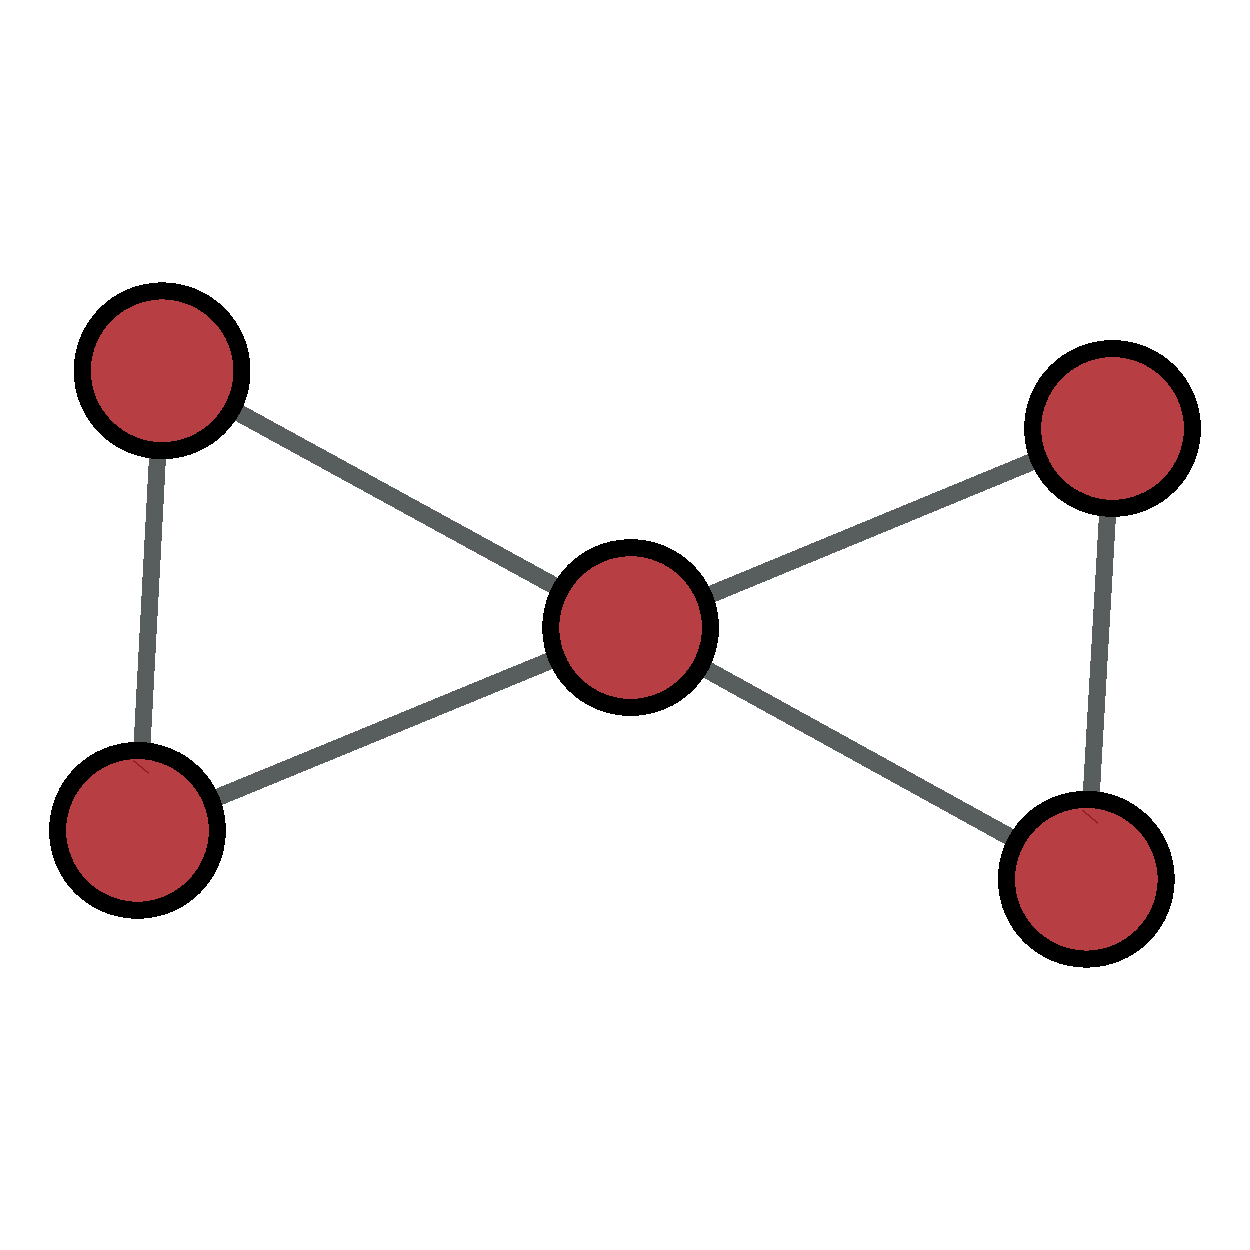
\includegraphics[width=0.5\columnwidth]{small_graph1.pdf}
\end{frame}
%-------------------------
%-------------------------
\begin{frame}
    \frametitle{Graph partitioning}
    \centering
    Problem of dividing a graph in a given number of groups of given sizes such that the number of links between the groups is minimized

    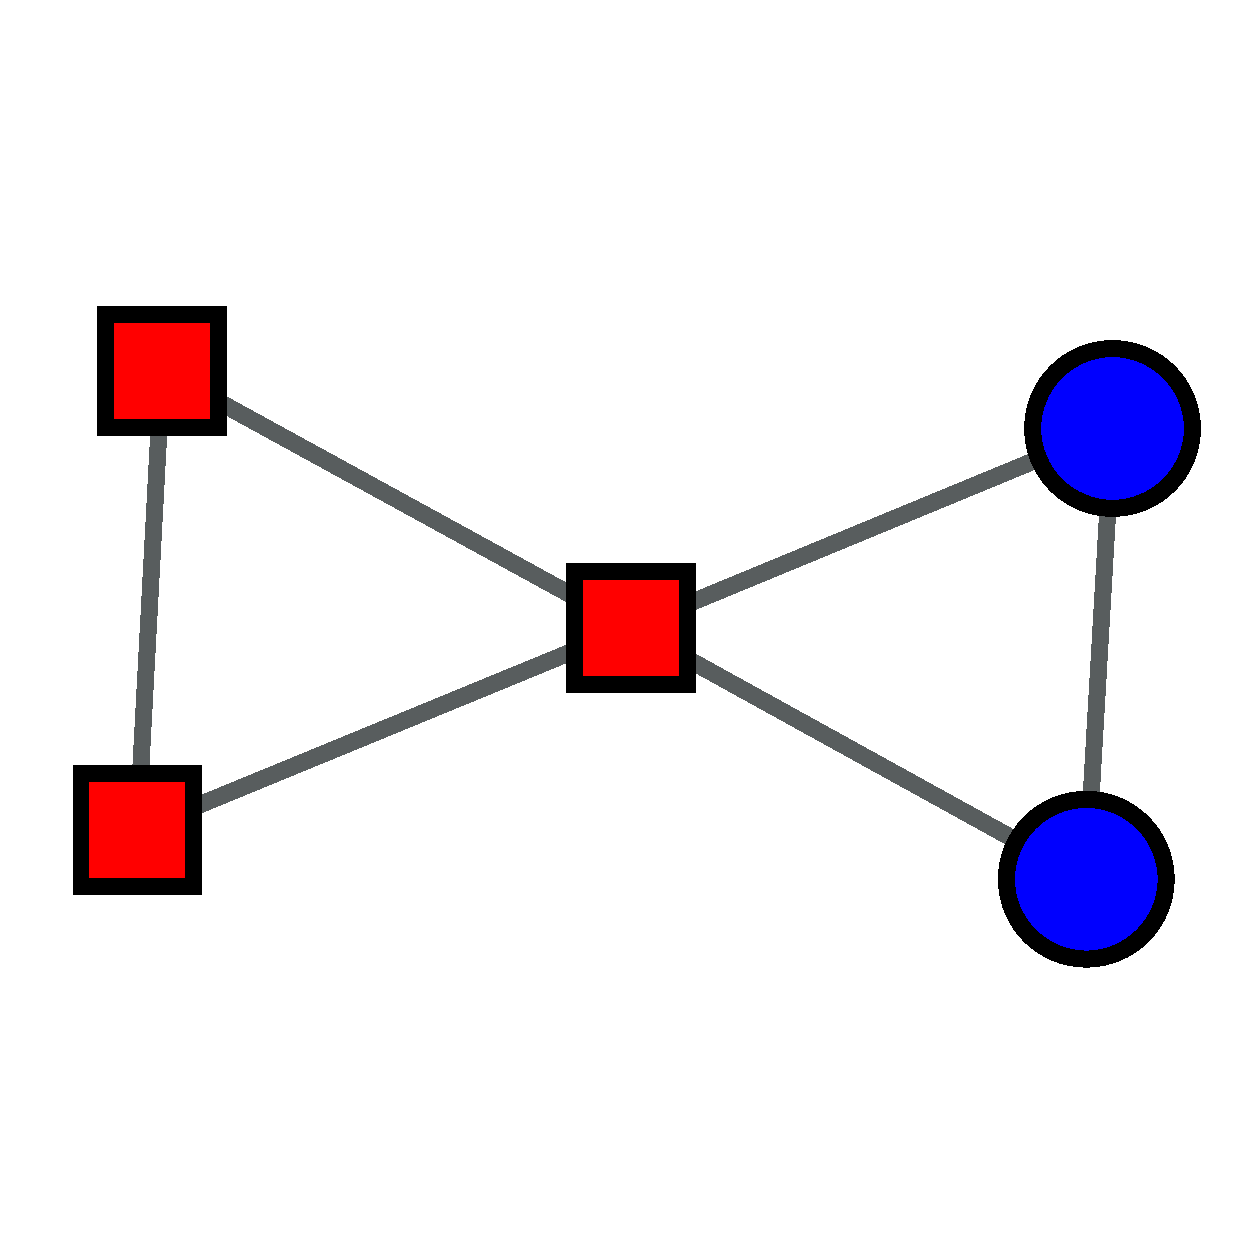
\includegraphics[width=0.5\columnwidth]{small_graph2.pdf}
\end{frame}
%-------------------------
%-------------------------
\begin{frame}
    \frametitle{Partitioning is hard!}
   \centering 
    \begin{itemize}
    \setlength\itemsep{1em}
        \item{Graph with $n$ vertices}
        \item{Find two groups with sizes $n_1$ and $n_2$ such that the cut size is minimum}
        \item{Number of ways: $\frac{n!}{n_1!n_2!}\approx \frac{2^{n+1}}{\sqrt{n}}$}
    \end{itemize}
    \centering
\end{frame}
%-------------------------
%-------------------------
\begin{frame}
    \frametitle{Community detection is harder!}
    \begin{itemize}
        \setlength\itemsep{2em}
        \item{{\bf Graph partitioning}
        \begin{itemize}
        \setlength\itemsep{0.5em}
            \item{\small well defined}
            \item{\small Number of groups is fixed}
            \item{\small Sizes of the groups are fixed}
            \item{\small Divide even if no good division exists}
        \end{itemize}
        }
        \item{{\bf Community detection}
        \begin{itemize}
        \setlength\itemsep{0.5em}
            \item{ill-defined}
            \item{\small Number of groups depends on the structure of the network}
            \item{\small Sizes of the groups depend on the structure of the network}
            \item{\small Discover natural fault lines}
        \end{itemize}
        }
    \end{itemize}
\end{frame}
%-------------------------
%-------------------------
\begin{frame}
    \frametitle{Too many algorithms}
    \centering
    \begin{itemize}
            \note<1>{I can go on}
    \setlength\itemsep{1em}
        \item{Girvan-Newman algorithm}
        \item{Modularity maximization}
        \item{Spectral decomposition}
        \item{Clique-percolation}
        \item{Radom walk methods}
        \item{Statistical inference}
        \item{Label propagation}
        \item{Hierarchical clustering}
    \end{itemize}
\end{frame}
%-------------------------
%-------------------------
\begin{frame}
    \frametitle{``The'' simplest community detection problem}
    \centering
    \begin{itemize}
    \setlength\itemsep{1em}
        \item{Bisecting a graph with $n$ nodes}
        \item{Group sizes are not fixed}
        \item{Minimum cut size?}
            \note<1>{Empty group}
    \end{itemize}
    \note<2>{Different measure}

    \vspace{2em}
    \pause
    {\bf A different measure of the quality of division is required..}
\end{frame}
%-------------------------
%-------------------------
\begin{frame}
    \frametitle{Quantification of community structure}
    \centering

    \begin{itemize}
        \setlength\itemsep{1em}
        \item{Fewer than expected edges between the groups}
            \note<1>{few edges = expected edges = not a good division}
            \note<2>{Remember assortativity}
            \pause
        \item{Equivalently, more than expected edges inside the groups}
            \pause
            \note<3>{Divide network using modularity}
        \item{Assortativity mixing and modularity}
            \pause
        \item{Look for divisions with high modularity}
            \note<4>{Heuristics are needed}
            \pause
        \item{Modularity maximization is hard}
    \end{itemize}

\end{frame}
%-------------------------
%-------------------------
\begin{frame}
    \frametitle{Heuristic algorithms for modularity maximization}
    \centering
    \begin{itemize}
        \setlength\itemsep{2em}
        \item{{\bf Agglomerative algorithms:}
            
    \begin{itemize}
        \setlength\itemsep{1em}
        \item{Hierarchical clustering}
        \item{Louvain method}
        \item{CNM algorithm}
    \end{itemize}
            
            }
        \item{{\bf Divisive algorithms:}
            
    \begin{itemize}
        \setlength\itemsep{1em}
        \item{Girvan-Newman algorithm}
        \item{Radichhi algorithm}
    \end{itemize}
            
            
            }
    \end{itemize}
\end{frame}
%-------------------------
%-------------------------
\begin{frame}
    \frametitle{Newman-Girvan algorithm}
    \centering
    
    \begin{itemize}
        \setlength\itemsep{1em}
        \item{Look for edges between the communities}

            %\note<1>{Number of shortest paths that pass through a given edge}
            \note<1>{Let's have a look at the edge betweenness}
        \item{Edge betweenness}
    \end{itemize}
\end{frame}
%-------------------------
%-------------------------
\begin{frame}
    \frametitle{}
    \centering
\end{frame}
%-------------------------
%-------------------------
\begin{frame}
    \frametitle{}
    \centering
\end{frame}
%-------------------------
%-------------------------
\begin{frame}
    \frametitle{}
    \centering
\end{frame}
%-------------------------
%-------------------------
\begin{frame}
    \frametitle{}
    \centering
\end{frame}
%-------------------------
%-------------------------
\begin{frame}
    \frametitle{}
    \centering
\end{frame}
%-------------------------
%-------------------------
\begin{frame}
    \frametitle{}
    \centering
\end{frame}
%-------------------------
%-------------------------
\begin{frame}
    \frametitle{}
    \centering
\end{frame}
%-------------------------
%-------------------------
\begin{frame}
    \frametitle{}
    \centering
\end{frame}
%-------------------------
%-------------------------
\begin{frame}
    \frametitle{}
    \centering
\end{frame}
%-------------------------
%-------------------------
\begin{frame}
    \frametitle{}
    \centering
\end{frame}
%-------------------------
%-------------------------
\begin{frame}
    \frametitle{}
    \centering
\end{frame}
%-------------------------
%-------------------------
\begin{frame}
    \frametitle{}
    \centering
\end{frame}
%-------------------------
%-------------------------
\begin{frame}
    \frametitle{}
    \centering
\end{frame}
%-------------------------
%-------------------------
\begin{frame}
    \frametitle{}
    \centering
\end{frame}
%-------------------------
%-------------------------
\begin{frame}
    \frametitle{}
    \centering
\end{frame}
%-------------------------
%-------------------------
\begin{frame}
    \frametitle{}
    \centering
\end{frame}
%-------------------------
%-------------------------
\begin{frame}
    \frametitle{}
    \centering
\end{frame}
%-------------------------
%-------------------------
\begin{frame}
    \frametitle{}
    \centering
\end{frame}
%-------------------------
%-------------------------
\begin{frame}
    \frametitle{}
    \centering
\end{frame}
%-------------------------
%-------------------------
\begin{frame}
    \frametitle{}
    \centering
\end{frame}
%-------------------------
%-------------------------
\begin{frame}
    \frametitle{}
    \centering
\end{frame}
%-------------------------
%-------------------------
\begin{frame}
    \frametitle{}
    \centering
\end{frame}
%-------------------------
%-------------------------
\begin{frame}
    \frametitle{}
    \centering
\end{frame}
%-------------------------
%-------------------------
\begin{frame}
    \frametitle{}
    \centering
\end{frame}
%-------------------------
%-------------------------
\begin{frame}
    \frametitle{}
    \centering
\end{frame}
%-------------------------
%-------------------------
\begin{frame}
    \frametitle{}
    \centering
\end{frame}
%-------------------------
%-------------------------
\begin{frame}
    \frametitle{}
    \centering
\end{frame}
%-------------------------
%-------------------------
\begin{frame}
    \frametitle{}
    \centering
\end{frame}
%-------------------------
%-------------------------
\begin{frame}
    \frametitle{}
    \centering
\end{frame}
%-------------------------
%-------------------------
\begin{frame}
    \frametitle{}
    \centering
\end{frame}
%-------------------------
%-------------------------
\begin{frame}
    \frametitle{}
    \centering
\end{frame}
%-------------------------
\end{document}
